% $Header: /Users/joseph/Documents/LaTbibeX/beamer/solutions/conference-talks/conference-ornate-20min.en.tex,v 90e850259b8b 2007/01/28 20:48:30 tantau $
%\documentclass{beamer}
\documentclass[handout]{beamer}
\usepackage{pgfpages}
% These slides also contain speaker notes. You can print just the slides,
% just the notes, or both, depending on the setting below. Comment out the want
% you want.
\setbeameroption{hide notes} % Only slides
%\setbeameroption{show only notes} % Only notes
%\setbeameroption{show notes on second screen=right} % Both
% Give a slight yellow tint to the notes page
\setbeamertemplate{note page}{\pagecolor{yellow!5}\insertnote}\usepackage{palatino}
\usefonttheme{professionalfonts} % using non standard fonts for beamer
  %\usefonttheme{serif}
% This file is a solution template for:
% -l Talk at a conference/colloquium.
% - Talk length is about 20min.
% - Style is ornate.
% Copyright 2004 by Till Tantau <tantau@users.sourceforge.net>.
%
% In principle, this file can be redistributed and/or modified under
% the terms of the GNU Public License, version 2.
%
% However, this file is supposed to be a template to be modified
% for your own needs. For this reason, if you use this file as a
% template and not specifically distribute it as part of a another
% package/program, I grant the extra permission to freely copy and
% modify this file as you see fit and even to delete this copyright
% notice. 
\mode<presentation>
{
  \usetheme{Warsaw} 
  \usecolortheme{crane}
  % or ...
  \setbeamercovered{transparent}
  % or whatever (possibly just delete it)
}
\usepackage{fontspec}
\setmainfont{Liberation Sans}
\setmonofont{Liberation Mono}

\usepackage[labelformat=empty]{caption}
\usepackage{hyperref}
\usepackage{xcolor}
\hypersetup{colorlinks=true, urlcolor=blue}
\title % (optional, use only with long paper titles)
[Developing the Cornish Dictionary]
{Developing the Cornish Dictionary using open source tools and data}
\author % (optional, use only with lots of authors)
{Davydh Trethewey}%\inst{1}}
% - Give the names in the same order as the appear in the paper.
% - Use the \inst{?} command only if the authors have different
%   affiliation.
\institute % (optional, but mostly needed)
{Project Support Assistant, Sodhva Kernewek - Cornish Language Office \\ 
Konsel Kernow - Cornwall Council \\
davidtreth@gmail.com \\ \href{http://taklowkernewek.neocities.org}{taklowkernewek.neocities.org}}
\date[WikiCelticKnot2019] % (optional, should be abbreviation of conference name)
{Keskusulyans Wikimedia Kolm Keltek - Wikimedia Celtic Knot conference,\\ 5th July 2019, Penryn Campus}
% - Either use conference name or its abbreviation.
% - Not really informative to the audience, more for people (including
%   yourself) who are reading the slides online
% If you have a file called "university-logo-filename.xxx", where xxx
% is a graphic format that can be processed by latex or pdflatex,
% resp., then you can add a logo as follows:
% \pgfdeclareimage[height=0.5cm]{university-logo}{university-logo-filename}
% \logo{\pgfuseimage{university-logo}}
% Delete this, if you do not want the table of contents to pop up at
% the beginning of each subsection:
%\AtBeginSubsection[]
%{
%  \begin{frame}<beamer>{Outline}
%    \tableofcontents[currentsection,currentsubsection]
%  \end{frame}
%}
% If you wish to uncover everything in a step-wise fashion, uncomment
% the following command: 
%\beamerdefaultoverlayspecification{<+->}
\usepackage[backend=biber]{biblatex}
\renewcommand*{\bibfont}{\footnotesize}
\addbibresource{wikimedia2019-gerlyver-warlinenn.bib}
\begin{document}
\begin{frame}
  \titlepage
\note[item]{If there's anything to add to the chair's introduction of me, do so now}  
\end{frame}
\section{Previous Dictionary}
\subsection{Previous Cornish dictionary website}
\begin{frame}{Previous Online Dictionary}
  % - A title should summarize the slide in an understandable fashion
  %   for anyone how does not follow everything on the slide itself.
  \begin{itemize}  
  \item Standard Written Form of Cornish online dictionary \href{https://web.archive.org/web/20190324085922/http://www.cornishdictionary.org.uk/cornish/alpha}{cornishdictionary.org.uk} (Internet Archive Wayback Machine)
  \end{itemize}
  \begin{figure}
 \begin{center}
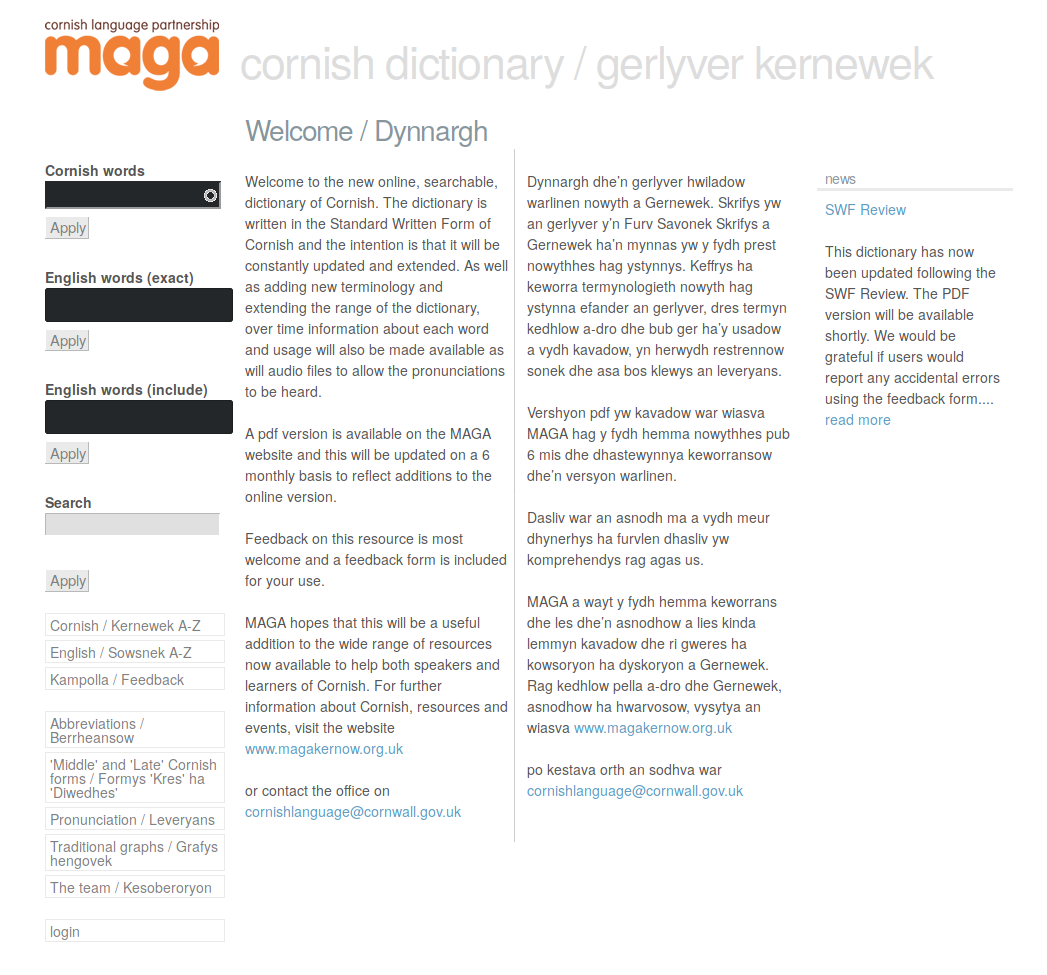
\includegraphics[width=6cm]{cornishdictionarywebsite.png}
 \end{center}
 \caption{}
 \label{fig:SWFdict_screenshot}
\end{figure}
\note[item]{This was the previous website up to June 2019}
\note[item]{Different search boxes for English-Cornish and Cornish-English}
\end{frame}
\subsection{Improvements to the dictionary}
\begin{frame}{Features in an ideal online dictionary}
\begin{itemize}
 \item<1-> Improve usability on different platforms desktop/tablet/mobile
 \item<2-> Cater for the various users of the language, including users of different varieties of Cornish
 \item<3-> Show personal forms for verbs and prepositions
 \item<4-> Ability to add sound samples
 \item<5-> Disambiguation of translation equivalents
\end{itemize}
\note[item]{Previous version could be cumbersome to use on mobile platforms. Maes T uses Google Web Toolkit allowing a responsive web-based interface. Maes T allows the backend data to be separated from the frontend website, for Welsh this has allowed use on different websites and mobile apps using an API. The Language Technologies Unit in Bangor has created a Wordpress plugin {\it Porthydd} to assist its deployment.\cite{prys2012distributing}}
\note[item]{Note difference between Middle and Late forms. \\ needs of beginning learners,
advanced learners, fluent speakers, Akademi members doing language development work.}
\note[item]{Personal forms were done for prepositions, which combine with personal pronouns in Cornish to form inflected forms. \\
hasn't been done for verbs, since this is a larger set of words, several tenses for each verb.
perhaps show the most common paradigms and the auxilliary verbs?}
\note[item]{Having sound samples is probably better than using IPA\\
beginners may not understand these symbols.
some of them aren't really agreed on, it is a Standard Written Form and
may not be prescriptive for pronunciation.}
\note[item]{e.g. \href{http://www.cornishdictionary.org.uk/?locale=en\#understanding}{understanding} can mean an agreement, or knowledge. note dictionary also matches verb form understand, this is a feature of Maes T.}
\end{frame}
\begin{frame}{Things to improve}
\begin{itemize}
 \item<1-> English to Cornish, and Cornish to English had been separately created in previous version
 \item<2-> Some errors and inconsistencies
 \item<3-> Updates according to 2013 review of the Standard Written Form
 \item<4-> Integration of work done by Terminology Panel of Akademi Kernewek
 \item<5-> Provide platform for further work by Akademi Kernewek
\end{itemize}
\note[item]{Previous version had been done in a software called TshwaneLex.}
\note[item]{Some review updates had already been done in the previous software, but not all.}
\note[item]{Terms standardised by the Terminology Panel and recommended for use.}
\note[item]{Akademi has a process for proposing a term, and wanted to be able to place it online but marked as a `proposed term' so that the community would be able to comment on it
before it became an established word in the language. There is a similar process in Maes T for Welsh, but this is within the group of domain experts prior to online publication.}
\end{frame}
\section{The Data in XML format}
\subsection{Analysis using Python}
\begin{frame}{Dictionary data}
 \begin{itemize}
  \item<1-> Exported from the software used in the previous version as an XML file
  \item<2-> Each word or phrase in the dictionary is a $<$lemma$>$ tag group
  \item<3-> Various information in sub-tags
  \item<4-> e.g. pronunciation, part of speech, plural, English glosses, example sentence, etymology, attestations in the traditional texts  
 \end{itemize}
 \note[item]{XML is eXtensible Markup Language, which works along a similar principle to Hyper Text Markup Language, which web pages are written in, but being extensible, any text can be used as tag names.}
 \end{frame}
\begin{frame}{Tidying the XML}
\begin{itemize}
  \item<1-> Use Python \href{https://www.crummy.com/software/BeautifulSoup/}{Beautiful Soup} to analyse the XML
  \item<2-> Allows any errors or inconsistencies to be spotted by looping through the $<$lemma$>$s in the dictionary     
  \item<3-> Simplify some of the structure, move subentries to their own $<$lemma$>$s
  \item<4-> Collaboration with Dewi Bryn Jones (Bangor University) to enable it to be in a format suitable for import into Maes T
\end{itemize}
\note[item]{Certain words / phrases were in $<$partofspeechgroup$>$ and $<$subentry$>$ tags within $<$lemma$>$s.
   this could lead to duplication where one phrase could exist as subentries of more than one $<$lemma$>$}
\note[item]{Check cases where no part of speech is defined etc.}
\note[item]{Count occurances of descendant tags of $<$lemma$>$.}
\note[item]{Count how many $<$lemma$>$ have each part of speech.}
\end{frame} 
\begin{frame}{Variants within the language}
\begin{itemize}
\item<1-> Cornish as a revived language derives from sources at different time epochs
\item<2-> Broadly speaking, two time periods of Middle and Late Cornish
\item<3-> Different groups within the revival have based the revived language primarily on Middle or Late sources
\item<4-> Orthographic decisions have sometimes made these seem further apart than they really are
\end{itemize}
\note[item]{One of the major data processes undertaken by DT was to combine each word into a single $<$lemma$>$
and define the M and L variants where they exist within this.}
\note[item]{Previously they lived in independent $<$lemma$>$ and if you searched the M version it relied on references tags having been added to refer to the L version.}
\note[item]{The previous data was not always systematic about how M / L distinction was marked. The M and L forms were independent of each other.}
\end{frame}
%\begin{frame}[fragile]{Example of XML with M/L distinction}
%\begin{scriptsize}
%\href{http://www.cornishdictionary.org.uk/?locale=en#aswa}{aswa}
%\begin{semiverbatim}
%\color{gray}
%<lemma>
%<lemma.middlelemmasign>
%<middlespelling>{\color{black}aswa}</middlespelling>
%</lemma.middlelemmasign>
%<lemma.latelemmasign>
%<latespelling>{\color{black}ajwa}</latespelling>
%</lemma.latelemmasign>
%<lemma.middlepronunciation>['azwa]</lemma.middlepronunciation>
%<lemma.latepronunciation>['æʤ(w)ɐ]</lemma.latepronunciation>
%<lemma.partofspeech>{\color{black}n.f}</lemma.partofspeech>
%<lemma.middleplural>{\color{black}aswaow}</lemma.middleplural>
%<lemma.lateplural>{\color{black}ajwaow}</lemma.lateplural>
%<sense><te><te.te>{\color{black}breach}</te.te></te></sense>
%<sense><te><te.te>{\color{black}gap}</te.te></te></sense>
%</lemma>
%\end{semiverbatim}
%\end{scriptsize}
%\note[item]{On the website you can click through to the L version and vice versa, and to the English glosses.}
%\end{frame}
%\begin{frame}[fragile]{Example of XML with no M/L distinction}
%\begin{scriptsize}
%\href{http://www.cornishdictionary.org.uk/?locale=en#a-ugh}{a-ugh}
%\begin{semiverbatim}
%\color{gray}
%<lemma>
%<lemma.lemmasign>
%<spelling>{\color{black}a-ugh}</spelling>
%<homonymnumber>{\color{black}(1)}</homonymnumber>
%</lemma.lemmasign>
%<lemma.middlepronunciation>[a'y:x]</lemma.middlepronunciation>
%<lemma.latepronunciation>[ə'ɪʊʰ]</lemma.latepronunciation>
%<lemma.partofspeech>{\color{black}adv}</lemma.partofspeech>
%<sense><te><te.te>{\color{black}above}</te.te></te></sense>
%</lemma>
%\end{semiverbatim}
%\end{scriptsize}
%\note[item]{In this case there is only one spelling which is used by both Middle and Late Cornish. \\
%There is however a $<$homonymnumber$>$ tag because {\scriptsize \tt a-ugh} can also be a preposition, which is listed as a separate $<$lemma$>$.}
%\end{frame}
%\begin{frame}[fragile]{Example of XML - a-ugh (2)}
%\begin{tiny}
%\href{http://www.cornishdictionary.org.uk/?locale=en#a-ugh}{a-ugh}
%\begin{semiverbatim}
%\color{gray}
%<lemma>
%<lemma.lemmasign>
%<spelling>{\color{black}a-ugh}</spelling>
%<homonymnumber>{\color{black}(2)}</homonymnumber>
%</lemma.lemmasign>
%<lemma.partofspeech>{\color{black}prp}</lemma.partofspeech>
%<sense><te><te.te>{\color{black}above}</te.te></te></sense>
%<sense><te><te.te>{\color{black}over}</te.te></te></sense>
%<lemma.personal.forms>
%<sg1p>a-ughov</sg1p>
%<sg2p>a-ughos</sg2p>
%<sg3pm>a-ughto</sg3pm>
%<sg3pf>a-ughti</sg3pf>
%<pl1p>a-ughon</pl1p>
%<pl2p>a-ughowgh</pl2p>
%<pl3p>a-ughta</pl3p>
%</lemma.personal.forms>
%<lemma.late.personal.forms>...</lemma.late.personal.forms>
%</lemma>
%\end{semiverbatim}
%\end{tiny}
%\note[item]{The preposition homonym has personal forms listed.}
%\note[item]{There is also a $<$lemma.late.personal.forms$>$ tag group which was edited out on the slide for brevity containing the Late personal forms.}
%\end{frame}
\subsection{Importing to Maes T}
\begin{frame}{Maes T software}
\begin{itemize}
\item<1-> Software that is used for terminology dictionaries in Welsh online at \href{http://termau.cymru/}{http://termau.cymru}
\item<2-> Developed by \href{https://www.bangor.ac.uk/canolfanbedwyr/technolegau_iaith.php.en}{Language Technologies Unit}, Canolfan Bedwyr, Bangor University
\cite{andrews2016terminology} \cite{andrews2011maes}
\item<3-> Deployable via an API to the web or apps \cite{prys2012distributing} 
\item<4-> Maes T has also been used for \href{http://geiriadur.bangor.ac.uk}{geiriadur.bangor.ac.uk} and \href{http://www.termiaduraddysg.org/}{www.termiaduraddysg.org} where sound samples are also presented
\end{itemize}
\note[item]{Maes T was guided by ISO standard formats and practices for terminology and lexicography. The ISO standard 15188 recommends a working group of 5-8 subject specialists and a terminologist.\\Provide interface designed to be user-friendly to non-terminologists, bilingual English-Welsh.}
\note[item]{There is a four stage process\\1. Collecting Terms - record candidate terms for the source language term.\\2. Defining the concept - define in the source and target languages, add a disambiguator where needed.\\3. Standardizing Terms -record normative status of candidate terms.\\4. Linguistic Information - record part of speech, gender, plural forms etc.}
\note[item]{Data can be served via an API, features such as showing related entries, popups to explain pos tags. matching images from Wikidata, Wikimedia Commons, linking to Wikipedia.}
\note[item]{Potential benefits of ISO standard based approach of Maes T for Cornish, such as software locali$[$sz$]$ations.}
\end{frame}
%\begin{frame}{Termau.cymru}
%\begin{figure}
 %\begin{center}
%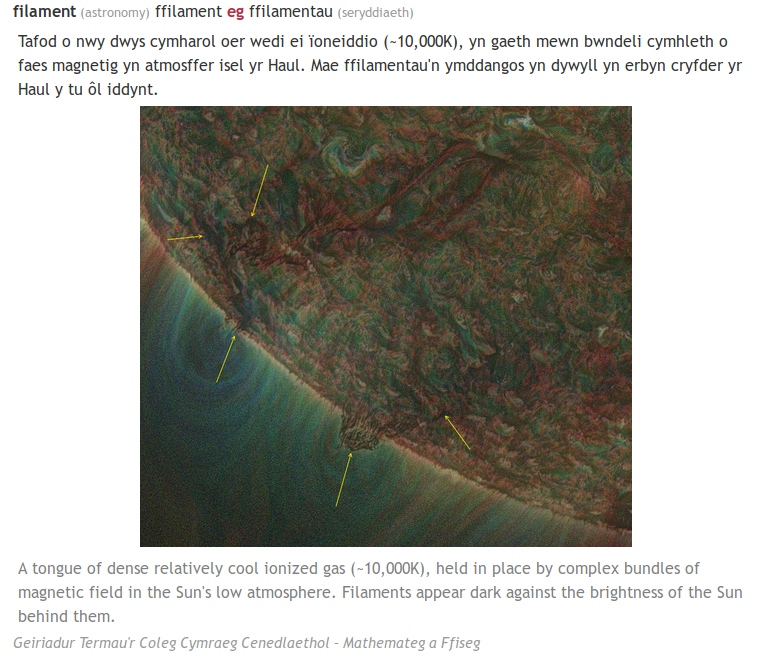
\includegraphics[width=6cm]{filament_solar.png}
 %\end{center}
 %\caption{\href{http://termau.cymru/\#filament}{termau.cymru/\#filament} \cite{Crossing2018}}
 %\label{fig:filament}
%\end{figure}
%\note[item]{Filament: \href{http://termau.cymru/\#filament}{termau.cymru/\#filament}. In this case, the image was contributed by an expert, along with a definition.}
%\end{frame}
%\begin{frame}{Termau.cymru}
%\begin{figure}
 %\begin{center}
%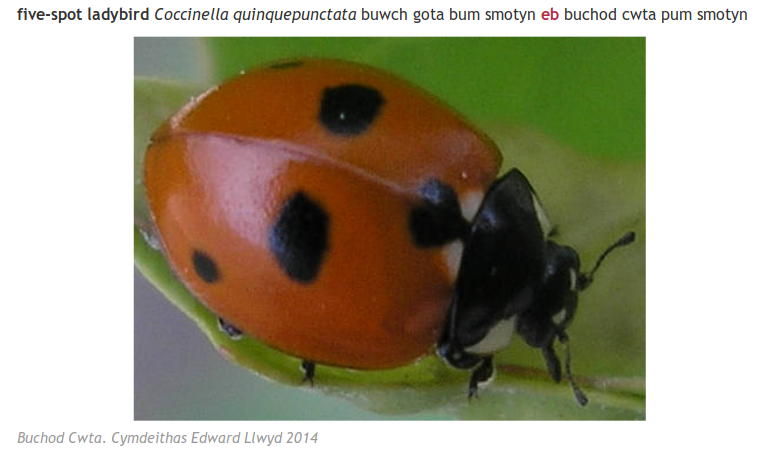
\includegraphics[width=8cm]{ladybird5spot.png}
 %\end{center}
 %\caption{\href{http://termau.cymru/\#ladybird}{termau.cymru/\#ladybird}}
 %\label{fig:ladybird}
%\end{figure}
%\note[item]{Ladybirds: \href{http://termau.cymru/\#ladybird}{termau.cymru/\#ladybird}. In this case, Wikimedia commons images were used (manually chosen during a project with \href{http://www.cymdeithasedwardllwyd.cymru}{\it Cymdeithas Edward Llwyd}).}
%\end{frame}
%\begin{frame}{Termau.cymru}
%\begin{figure}
 %\begin{center}
%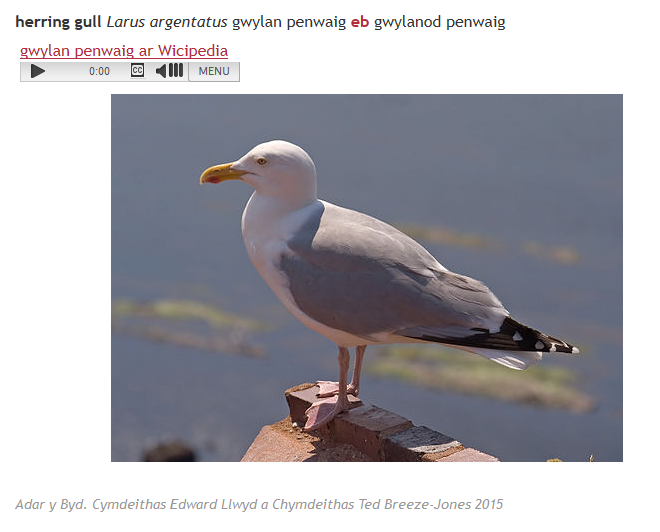
\includegraphics[width=7cm]{herringgull.png}
 %\end{center}
 %\caption{\href{http://termau.cymru/\#gull}{termau.cymru/\#gull}}
 %\label{fig:seagull}
%\end{figure}
%\note[item]{This was added as part of {\it Adar Y Byd}, a dictionary of bird names from \href{http://www.cymdeithasedwardllwyd.cymru}{\it Cymdeithas Edward Llwyd}. This had 9500 entries, so an automated method was used.}
%\note[item]{There is a species of moth called `Silurian' and this found a Wikimedia image of a Doctor Who character. \cite{Crossing2018}\\Note also: \href{http://termau.cymru/\#apple}{termau.cymru/\#apple} which showed as of July 2019 a picture of Apple headquarters rather than the fruit.}
%\end{frame}
\begin{frame}{Adapting Maes T to better serve Cornish}
\begin{itemize}
\item<1-> Collaboration with Dewi Bryn Jones to adapt the Maes T software for Cornish
\item<2-> Some relevant grammatical differences between Welsh and Cornish
\item<3-> Other changes come from using it for a general dictionary
website rather than terminology dictionaries that usually have a 1:1 correspondence between Welsh-English in a given context
\end{itemize}
\note[item]{The original purpose of Maes T was to support terminology dictionaries which aimed at a one to one mapping between source language and target language terms. Although it had been used since for more general dictionaries such as \href{http://geiriadur.bangor.ac.uk}{Geiriadur Bangor}.}
\note[item]{Welsh grammars tend to treat the singulative / collective nouns as a normal singular / plural distinction e.g. coeden - coed, plentyn - plant, where the noun loses an ending to become plural.}
\note[item]{The plural of the singulative is a feature of (at least some forms) of Cornish, for a number of individual items, rather than en masse, for at least some n.coll. E.g. gwydh, gwedhen, gwydhennow. Not currently shown in dictionary.} 
\end{frame}
\begin{frame}{Transition to editing within Maes T}
\begin{itemize}
\item<1-> Once the structure is stable, move away from manually editing XML to editing within Maes T
\item<2-> More practical for a wider range of people e.g. Dictionary Panel members of the Akademi Kernewek to edit
\item<3-> Manually editing an XML file can be error prone, which was mitigated by the
Python scripts validating / analysing it
\end{itemize}
\note[item]{In production, the data would be edited by a number of different people who may be non-programmers.}
\note[item]{Maes T can provide a platform for this in a similar way as to the Welsh terminology development.}
\end{frame}
\section{Application of the work}
\subsection{Terminology}
\begin{frame}{Terminology Panel}
\begin{itemize}
\item<1-> \href{http://www.akademikernewek.org.uk/}{Akademi Kernewek}, the Cornish language academy has a \href{https://akademikernewek.weebly.com/terminology.html}{terminology panel} to research new terms for the language
\item<2-> A number of subject areas have been considered so far: plants, insects, mining, minerals, architecture, grammar
\end{itemize}
\note[item]{Briefly outline process by which Akademi intends to do this, and terminology areas in development.}
\note[item]{\href{https://akademikernewek.weebly.com/uploads/7/8/1/9/78199260/ak_terminology_policy.pdf}{Akademi terminology policy} outlining process of creating a term.}
\note[item]{\href{https://akademikernewek.weebly.com/uploads/7/8/1/9/78199260/ak-dictionary-policy-13082018.pdf}{Akademi dictionary policy} according to which a terminology item is recommended and after a period of review becomes considered part of the main dictionary}
\end{frame}
\subsection{Linking to open-source data}
\begin{frame}{Using open source data from Wikimedia}
\begin{figure}
 \begin{center}
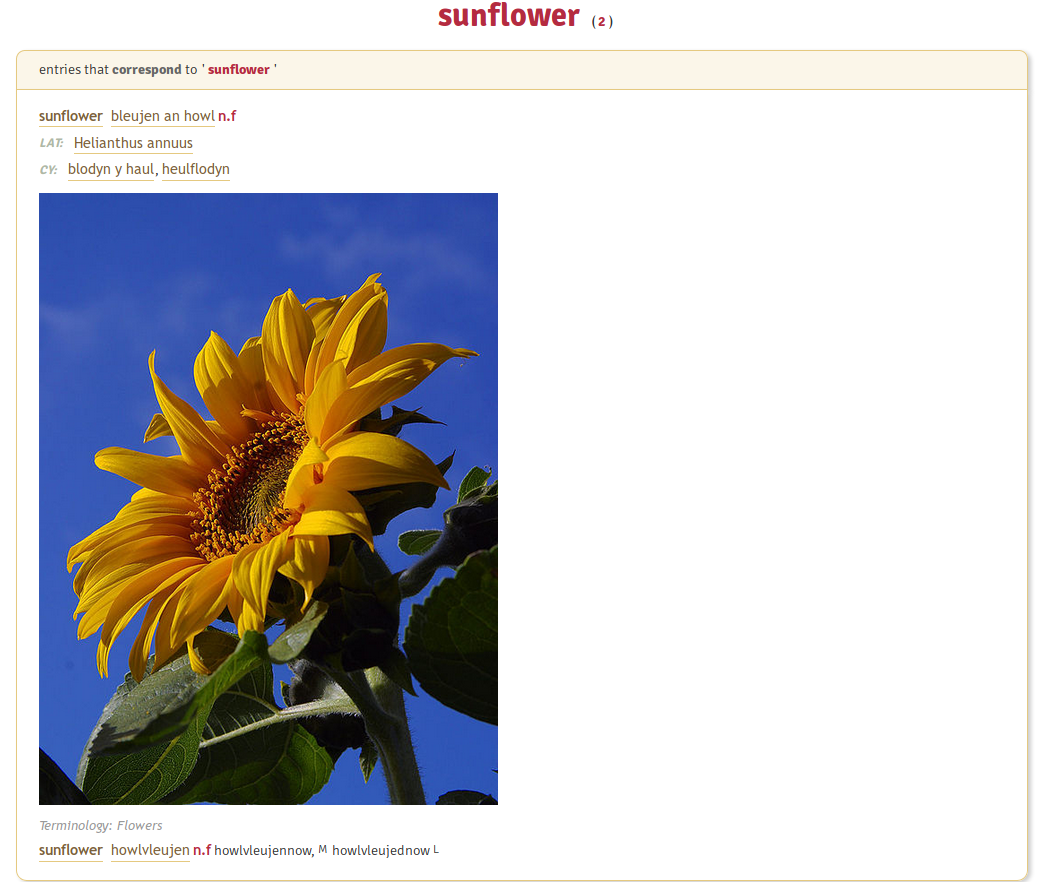
\includegraphics[width=7cm]{sunflower.png}
 \end{center}
 \caption{\href{http://www.cornishdictionary.org.uk/\#sunflower}{www.cornishdictionary.org.uk/\#sunflower} \cite{Crossing2018}}
 \label{fig:sunflower}
\end{figure}
\note[item]{Explain a bit about linking to Wikimedia Commons images of plants, and to Wikipedia.}
\note[item]{See \cite{Crossing2018} for more information on \href{http://termau.cymru}{Porth Termau Cenedlaethol Cymru} linking to Wikimedia images. This included automatically finding them using English and Latin names. }
\end{frame}
\subsection{Demonstration of new dictionary website}
\begin{frame}{New dictionary website}
\begin{itemize}
\item Demonstrate the new dictionary website (demo of \href{http://cornishdictionary.org.uk/test/}{cornishdictionary.org.uk}) 
\end{itemize}
\note[item]{New version is now at the main URL.}
\note[item]{Possibly do the demo at the end or in an unconference session subject to time, maybe better for flow of the talk to move to conclusions now.}
\note[item]{Responsive design - e.g. \href{http://cornishdictionary.org.uk/\#moon}{cornishdictionary.org.uk/\#moon} automatically switches to two-column layout where there are matches in both languages, and if the screen width is low, these are stacked vertically rather than side-by-side.}
\end{frame}
\section*{Summary}
\begin{frame}{Conclusions and future ideas}
  % Keep the summary *very short*.
\begin{itemize}
  \item<1-> We already have some example sentences, but could have many more of these, and audio of them by speakers
  \item<2-> Method of handling Middle and Late variants allows multiple variants to be supported while keeping them semantically as one
 $<$lemma$>$ item
 \end{itemize}
 \begin{scriptsize}
\note[item]{Other features that would be nice?}
\note[item]{Make plurals / singulatives searchable e.g. mergh, gwedhen \\ search aware of mutation such that `gath' finds `kath',\\
awareness of `traditional' spellings that some users prefer such that searching `cath' finds `kath' \\
spellings from other forms of Cornish e.g. gwydhenn (Kemmyn) - gwedhen (SWF) \\
could M / L, and/or the `traditional' forms be offered as a user selection at the front-end?\\
and a choice between a strict and `fuzzy' search?}
\note[item]{Maes T does this for Welsh, using lemmatizers, spelling and grammar checkers. e.g. \href{http://geiriadur.bangor.ac.uk/\#plant}{geiriadur.bangor.ac.uk/\#plant} lemmatizes `plant' to the singular `plentyn' ``child''. It will also present the English entries for `plant'. \href{http://geiriadur.bangor.ac.uk/\#mor}{geiriadur.bangor.ac.uk/\#mor} gives the conjunction/adverb mor and the noun môr, as well as bôr (an alternate spelling for bore, b could have nasal mutated to m).\\Maes T customizes results using different API keys including different terminology resources and search settings.}
\note[item]{Possibilities of wider linking to Wikimedia items including Wikidata?}
\note[item]{Linkage with place-name map?}
\end{scriptsize}
\end{frame}
\begin{frame}[plain]{References}
\printbibliography
%\note{\printbibliography}
\end{frame}
 %\begin{frame}[plain]{Possible things to talk about in unconference sessions}
 %\begin{itemize}
 %\item Another way of doing things would be to generate static HTML pages programatically from the XML, which I also did
%\item As a side project of this, I programatically matched the English glosses to Unicode character names
%\end{itemize}
%\end{frame}
%\begin{frame}[plain]{Cornish Emojis}
%\begin{figure}
 %\begin{center}
%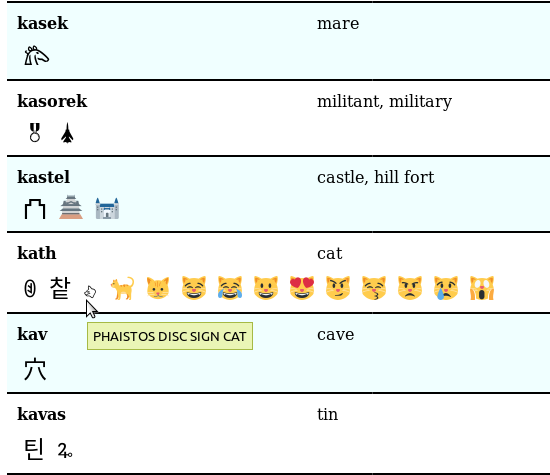
\includegraphics[width=7cm]{emojis_example.png}
 %\end{center}
 %\caption{\href{https://unicode-table.com/101ec}{Cat Emoji (circa 1500BC)} from the \href{https://unicode-table.com/en/blocks/phaistos-disc/}{Phaistos Disc}}
 %\label{fig:emojis}
%\end{figure}
%\note[item]{}
%\end{frame}
\end{document}
